\section{PID-Regler \formelbuch{142}}

\subsection{P-Regler -- Stationärer Zustand \formelbuch{147}}
Beim einfachsten linearen Regler, dem P-Typ, besteht ein proportionaler Zusammenhang zwischen Fehler $e$ und Stellgrösse $u$.
Der P-Regler reagiert schnell, kann aber den Sprungfehler nicht vollständig eliminieren.
Er hat einen stationären Fehler.
Eine zu hohe Verstärkung $K_R$ führt zu Rauschen.


\subsection{I-Regler \formelbuch{149}}
Der reine I-Regler ist allgemein ungünstig, weil er relativ langsam arbeitet und die Stabilität schwächt. Ist aber die Regelstrecke nur erster Ordnung, erzielt man gute Ergebnisse mit dem I-Regler.
Der I-Regler neigt zum Schwingen.
Bei sprungförmigen Signalen, d.h. für Festwertregelungen hat der I-Regler keinen Fehler!


\subsection{PI-Regler \formelbuch{150}}
\begin{figure}[h!]
	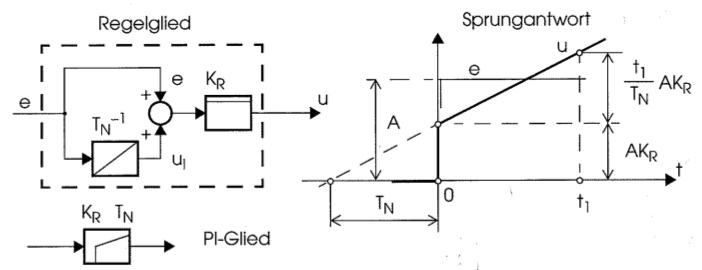
\includegraphics[width=\linewidth]{./images/PI_Regler.jpg}
\end{figure}
\begin{description}
	\item[Sprungantwort]
		\[
			u(t) = K_R\left( 1 + \frac{t}{T_N}\right)
		\]
	\item[\"Ubertragungsfunktion]
		\[
			G_\text{PI}(j\omega) = K_R \frac{1+j\omega T_N}{j\omega T_N}
		\]
\end{description}


\subsection{PD-Regler}
\begin{figure}[h!]
	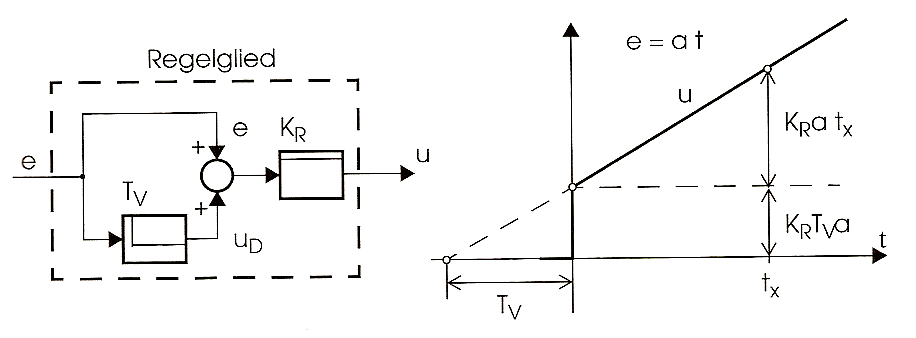
\includegraphics[width=\linewidth]{./images/PD_Regler.png}
\end{figure}
Der PD-Regler entspricht dem inversen PT\(_1\)-Glied. Meistens wird jedoch der PDT\(_1\) Regler verwendet.
\begin{description}
	\item[Rampenantwort]
		\[
			u(t) = K_R at + K_R T_V a \text{ wenn } e(t) = a\cdot t
		\]
	\item[Sprungantwort]
		\[
			u(t) = K_R \left( 1 + \frac{T_V}{T_C} \cdot e^{-t/T_C} \right)
			\text{ wenn } e(t) = 1(t)
		\]
	\item[\"Ubertragungsfunktion] \(T_V > T_C\)
		\[
			G_{\text{PDT}_1}(j\omega) = K_R \frac{1+j\omega(T_V+T_C)}{1+j\omega T_C}
		\]
\end{description}
 

\subsection{PIDT\(_1\)-Regler (Reeller PID) \formelbuch{153}}
Praktisch sind \(T_N \leq T_V\), \(T_C < T_V\) und \(T_C = T_V/(4\ldots \text{ bis }\ldots 50)\)

\subsubsection{Additive Form}
\begin{figure}[h!]
	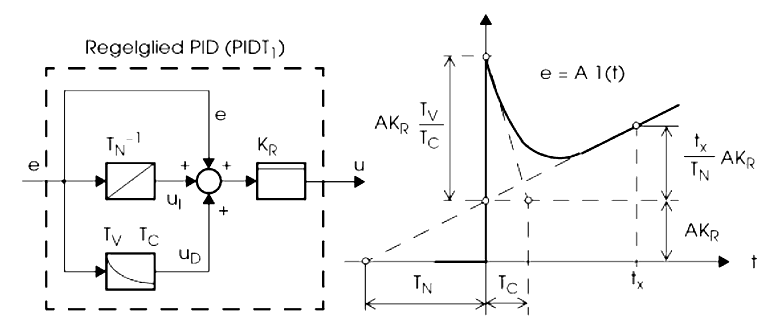
\includegraphics[width = \linewidth]{./images/PID_Regler_add}
\end{figure}
\begin{description}
	\item[\"Ubertragungsfunktion]
		\[
			G_{\text{PIDT}_1}^{+} (j\omega) = K_R \left(
				1 + \frac{1}{j\omega T_N} + \frac{j\omega T_V}{1 + j\omega T_C}
			\right)
		\]
	\item[Sprungantwort]
		\[
			u(t) = K_R \left( 1 + \frac{t}{T_N} + \frac{T_V}{T_C}e^{-t/T_C} \right)
		\]
\end{description}

\subsubsection{Multiplikative Form (Serienschaltung)}
\begin{figure}[h!]
	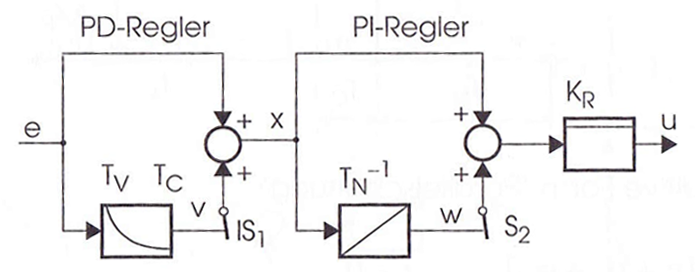
\includegraphics[width = \linewidth]{./images/PID_Regler_mul}
\end{figure}
\begin{description}
	\item[\"Ubertragungsfunktion]
		\[
			G_{\text{PIDT}_1}^{\times} (j\omega) = 
			K_R \cdot \frac{1 + j\omega T_N}{j\omega T_N}
			\cdot \frac{1 + j\omega (T_V + T_C)}{1 + j\omega T_C}
		\]
	\item[Sprungantwort]
		\[
			u(t) = K_R \left[ 
			1 + \frac{T_V}{T_N} +\frac{t}{T_N} + \left(
			\frac{T_V}{T_C}-\frac{T_V}{T_N}
			\right) e^{-t/T_C}
			\right]
		\]
\end{description}

\subsection{Empirische Einstellregeln \formelbuch{162}}
\begin{figure}[h!]
	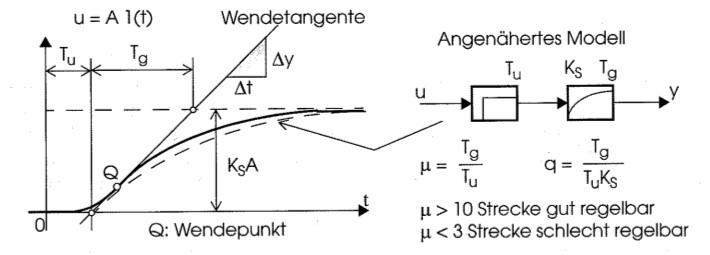
\includegraphics[width=\linewidth]{./images/Empirisch_Regeln.jpg}
\end{figure}
UTF des angenäherten Modells:
\[
	G_0(j\omega) = \frac{K_s}{1+j\omega T_g} e^{-j\omega T_u}
\]
Empirische Einstellregeln ergeben in der Praxis nicht immer das bestmögliche Zeitverhalten, sondern sie liefern eine erste Einstellung, welche experimentell noch verbessert werden kann.
  
Um Ausschläge im Stellsignal, welche durch die typische Reaktion eines DT\(_1\) auf einen Sprung verursacht werden, zu verhindern, darf man die Führungsgrösse \(r\) nicht über den Differenzierer leiten.

%% TODO: fix this table
\begin{table*}
	\renewcommand\arraystretch{1.2}
	\centering
	\begin{tabular}{ ll rrrrrr }
		\toprule
		\multicolumn{6}{l}{
			\textbf{Chien-Hrones-Reswick}
		}
		&
		\multicolumn{2}{l}{
			\textbf{Ziegler-Nichols}
		}
		\\ 

		\cmidrule(lr){1-6} \cmidrule(lr){7-8}
		\multicolumn{6}{l}{
			\(\displaystyle
				q = \frac{T_g}{T_uK_S}, \quad
				\mu = \frac{T_g}{T_u} \quad
				\text{wenn } \mu
				\begin{cases}
					> 10 & \text{Strecke gut regelbar} \\
					< 3  & \text{Strecke schlecht regelbar}
				\end{cases}
			\)
		}
		&
		\(\displaystyle q = \frac{T_g}{T_uK_s} \)
		&
		\(\displaystyle K_{R\pi}, \qquad T_\pi = \frac{2\pi}{\omega_\pi}\)
		\\

		\cmidrule(lr){1-6} \cmidrule(lr){7-8}

		\textbf{Regler}
		&
		% \textbf{Parameter}
		&
		\multicolumn{2}{p{3.5cm}}{
			\textbf{Führungsverhalten} % \newline $y_m$: Überschwingen
		}
		&
		\multicolumn{2}{l}{
			\textbf{Störverhalten}
		}
		&
		\multicolumn{1}{l}{
			\textbf{Sprungantwort}
		}
		&
		\multicolumn{1}{l}{
			\textbf{Stabilitätsgrenze}
		}
		\\

		\multicolumn{2}{l}{und Parameter}
		& kein $y_m$ & $y_m / y_\infty = 20 \%$ & kein $a$ & $a / b = 20 \%$ & & \\

		\cmidrule(lr){1-2}
		\cmidrule(lr){3-4}
		\cmidrule(lr){5-6}
		\cmidrule(lr){7-7}
		\cmidrule(lr){8-8}
		P & $K_R$ & $0.3q$ & $0.7q$ & $0.3q$ & $0.7q$ & $q$ & $0.5K_{R\pi}$ \\

		% \cmidrule(lr){1-6} \cmidrule(lr){7-8}
		PI & $K_R$ & $0.35q$   & $0.6q$ & $0.6q$ & $0.7q$    & $0.9q$    & $0.45K_{R\pi}$ \\
       & $T_N$ & $1.17T_g$ & $1T_g$ & $4T_u$ & $2.33T_u$ & $3.33T_u$ & $0.85T_{\pi}$  \\

		% \cmidrule(lr){1-6} \cmidrule(lr){7-8}
		PID & $K_R$ & $0.6q$   & $0.95q$   & $0.95q$   & $1.2q$    & $1.2q$   & $0.60K_{R\pi}$ \\
        & $T_N$ & $1T_g$   & $1.36T_g$ & $2.38T_u$ & $2T_u$    & $2T_u$   & $0.50T_\pi$    \\
        & $T_V$ & $0.5T_u$ & $0.47T_u$ & $0.42T_u$ & $0.42T_u$ & $0.5T_u$ & $0.125T_\pi$   \\
		\bottomrule
	\end{tabular}
	\caption{Empirische Reglereinstellung}
\end{table*}

\subsection{Wind-Up \formelbuch{170}}
\begin{description}
	\item[Definition] Der Fehler \(e\) am Integratoreingang bleibt konstant, sodass dessen Ausgangssignal ständig zunimmt.
	\item[Folge] Einerseits ein konstanter Fehler und andererseits eine verzögert reagierende und damit stark überschwingende Regelgrösse \(y\).

	\item[Ursachen]
		\begin{itemize}
			\item I-Anteil
			\item Sättigung am Regler-Ausgang
			\item \(e(t)\) über ``längere Zeit'' $\neq 0$
		\end{itemize}

	\item[Anti-Wind-Up] Integration beschränken.
\end{description}
